%% what_is_datavis.tex
%% Author: Leighton Pritchard
%% Copyright: James Hutton Institute
%% What is data visualisation

% STORYTELLING
\begin{frame}
  \frametitle{Data visualisation is art and science}
    $\ldots$storytelling in pictorial or graphical format \\
      \begin{itemize}  
        \item <1->\textcolor{hutton_green}{Stories to yourself (sense-making)}
        \begin{itemize}
          \item <2->summarise big stories quickly
          \item <2->data exploration and mining
          \item <2->identify areas/items of importance
          \item <2->find relationships and patterns
        \end{itemize}
        \item <1->\textcolor{hutton_blue}{Stories to others (communication)}
        \begin{itemize}
          \item <3->present your interpretation of data
          \item <3->make a specific point
          \item <3->assert a relationship or pattern
          \item <3->demonstrate significance
        \end{itemize}
        \item <1->\textcolor{hutton_purple}{Cautionary tales}
        \begin{itemize}
          \item <4->avoid distortion
          \item <4->make the reader think about the data, not the presentation
          \item <4->avoid \textit{chartjunk} (excessive decoration)
          \item <4->aim for high data:ink ratio
        \end{itemize}
      \end{itemize}  
\end{frame}


% WHAT IS THE POINT
\begin{frame}
  \frametitle{The point of data visualisation
  \footnote{\tiny{\href{https://en.wikipedia.org/wiki/Data_visualization}{https://en.wikipedia.org/wiki/Data\_visualization}}}
  }
    \textcolor{hutton_green}{Where does visualisation belong?}
    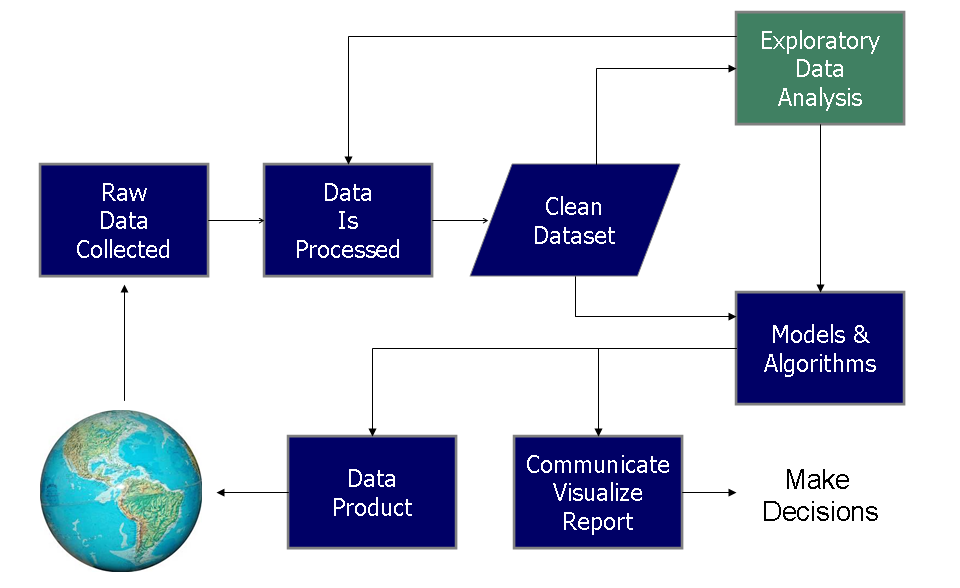
\includegraphics[width=\textwidth]{images/decisions}
\end{frame}


% EFFECTIVE COMMUNICATION
\begin{frame}
  \frametitle{Communicating effectively}
      \begin{itemize}  
        \item <1->\textcolor{hutton_green}{Understand the data}
        \begin{itemize}
          \item <2->size
          \item <2->cardinality
          \item <2->meaning
          \item <2->relationships
        \end{itemize}
        \item <1->\textcolor{hutton_blue}{Know (or be receptive to) the message}
        \begin{itemize}
          \item <3->what does pictorial representation mean?
          \item <3->match graphical relationships to data relationships
        \end{itemize}
        \item <1->\textcolor{hutton_purple}{Know your audience}
        \begin{itemize}
          \item <4->how do people process pictorial information
          \item <4->how does your audience process information
          \item <4->domain-specific representations
        \end{itemize}
      \end{itemize}  
\end{frame}


% Frame template 
\begin{frame}
  \frametitle{A model of communication
    \footnote{\tiny{\href{https://www.amazon.co.uk/Dont-Be-Such-Scientist-Substance}{Randy Olson (2009) \textit{Don't Be Such a Scientist}}}}
  }
  \begin{center}
    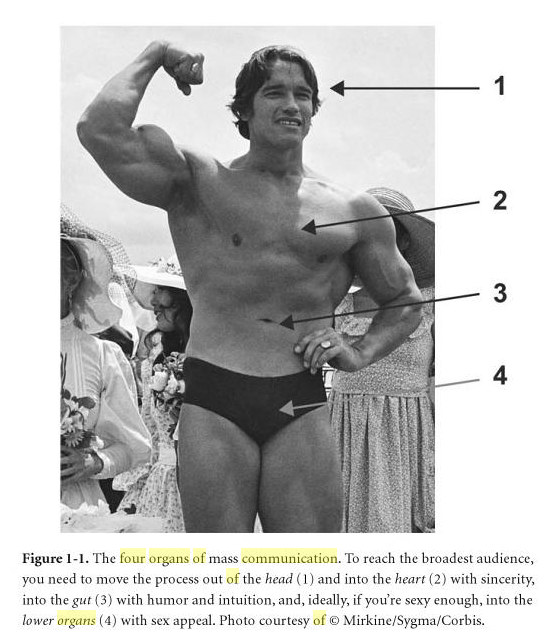
\includegraphics[height=0.8\textheight]{images/mass_communication_datavis}        
  \end{center}
\end{frame}